\chapter{线性 MPC 与约束跟踪}
\begin{notebox}
\textbf{目标}\quad 将受力模型、参考轨迹和线性约束写成 QP；只执行本次有效解的第一步。\\
\textbf{先修}\quad 第 04、13、14、17 章；yaw 仍使用独立前馈 + PD。
\end{notebox}
\section{把连续模型积分成预测矩阵}
\begin{lstlisting}[language=bash]
ros2 run motion2d mpc_demo tmp/ch18_mpc
/usr/bin/python3 scripts/plot_ch18_mpc.py
\end{lstlisting}
取 $x=[p_x,p_y,v_x,v_y]^\top$、$u=[F_x,F_y]^\top$，控制间隔为 $h$。
在一步内保持力不变，令 $\lambda=c_v/m$，$e=e^{-\lambda h}$，
$g=(1-e)/\lambda$，$f=(h-g)/\lambda$，则
\begin{equation}
 x_{k+1}=Ax_k+Bu_k,\qquad
 A=\begin{bmatrix}I&gI\\0&eI\end{bmatrix},\qquad
 B=\begin{bmatrix}(f/m)I\\(g/m)I\end{bmatrix}.
\end{equation}
$\lambda\to0$ 时 $g=h,f=h^2/2$。小阻力应使用第 04 章的稳定极限，避免两个相近数相减。
linearInertialModel 复用精确积分器的基向量响应来提取 A/B；输入取力限内的幅值后归一化。
控制与仿真共用动力学，测试另核对零阻力解析值。

重复代入 N 步，将未来状态和力依次堆叠为 $X=[x_1;\ldots;x_N]$、$U=[u_0;\ldots;u_{N-1}]$：
\begin{equation}
 X=S_xx_0+S_uU,\qquad (S_x)_k=A^k,\qquad
 (S_u)_{k,j}=\begin{cases}A^{k-1-j}B,&0\leq j<k,\\0,&j\geq k.\end{cases}
\end{equation}
预测步数与预测时间不同：$N=20,h=0.02$ s 只看未来 0.4 s。
位置与速度均在 odom，力单位 N。

\section{跟踪、前馈和输入变化组成一个二次型}
未来参考在 $t+h,\ldots,t+Nh$ 采样，前馈力 $U_r$ 由 $\hat m a_r+\hat c_vv_r$ 堆叠。
令 $D$ 为主对角 I、下一条块对角 $-I$ 的差分矩阵，$d=[u_{\rm previous};0;\ldots]$，代价为
\begin{equation}
 J=\|S_xx_0+S_uU-X_r\|_{\bar Q}^2+
 r\|U-U_r\|^2+s\|DU-d\|^2.
\end{equation}
$\bar Q$ 每步对位置与速度分别加权；$r>0$ 使力的二次型正定。
写成 $\tfrac12U^TPU+q^TU+\mathrm{const}$ 后，
\begin{align}
 P&=2(S_u^T\bar Q S_u+rI+sD^TD),\\
 q&=2\{S_u^T\bar Q(S_xx_0-X_r)-rU_r-sD^Td\}.
\end{align}
上一拍必须用\textbf{实际施加的力}，包括制动输入；不能用旧参考或未限幅请求替代。

\clearpage
\section{把约束按行装进矩阵}
求解器的统一形式为 $l\leq C U\leq u$，这里 C 是约束矩阵，避免与动力学 A 混淆。
分别堆叠以下线性行：
\begin{itemize}
\item 力：$-F_{\max}\leq U_i\leq F_{\max}$；两个方向独立。
\item 变化率：$-\dot F_{\max}h\leq DU-d\leq\dot F_{\max}h$，单位 N。
\item 速度：从 $S_xx_0+S_uU$ 取出各步速度，限制两个分量。
\item 走廊：每步选择已验证的配置空间凸区，代入 $H_kp_k\leq b_k$。
\end{itemize}
输入 N 个凸区与 N 个预测状态一一对应；区域已经考虑圆盘半径，不再膨胀一次。
这些约束只限制预测节点，不证明节点之间、定位误差下或跟踪偏离后的连续安全。
ESDF 是非线性距离场，若直接加入非线性约束，就需要另讲 SQP/NMPC，不能继续称作此处的线性 QP。
\lstinputlisting[language=C++,linerange={mpc_condense_begin-mpc_condense_end},includerangemarker=false]{../ros2_ws/src/motion2d/src/control/linear_mpc.cpp}

\section{看得懂的 ADMM 求解器}
本课程独立实现小型稠密正定 QP 求解器，不调用 OSQP 库。
它采用分裂变量 z 将线性系统求解与区间投影分开，主要参考
\href{https://osqp.org/docs/solver/index.html}{OSQP 官方算法说明}，省去稀疏排序、自动缩放和抛光等工程功能。
\lstinputlisting[language=C++,linerange={qp_admm_begin-qp_admm_end},includerangemarker=false]{../ros2_ws/src/motion2d/src/optimization/box_qp.cpp}
这里 solve 使用缓存的 LDLT 分解；每 25 次迭代按归一化残差调整 $\rho$，变化足够大时重新分解。
只有原始残差 $CU-z$ 与对偶残差 $PU+q+C^Ty$ 均满足绝对/相对容差才返回 solved。
默认容差均为 $10^{-5}$、最多 1500 次；无约束测试对照解析解 $-P^{-1}q$。

\clearpage
\section{失败状态与短时域的边界}
成功后仅施加 $u_0$；下一次重读状态、重建 QP。
上次成功 U 左移一块、重复尾块，作为本次初值；失败立即清空热启动并生成新的限幅阻尼力。
稠密构建、分解和迭代适合本章小问题，不承诺硬实时。
\begin{center}\small
\begin{tabular}{lp{9cm}}\toprule
状态 & 可得结论\\\midrule
solved & 残差在设定容差内；不是连续碰撞或闭环稳定性证明\\
primal\_infeasible & 上下界矛盾，或找到近似归一化不可行证书\\
max\_iterations & 给定迭代数内没收敛；不能因此断言问题不可行\\
time\_limit & 迭代间检查到墙钟预算用完；当前迭代可超出预算\\
numerical\_failure & 非有限迭代；不能继续使用该输入序列\\\bottomrule
\end{tabular}
\end{center}
不可行证书满足 $C^Tv\approx0$ 且 $u^Tv_++l^Tv_-<0$；非有限单侧边界不能参与错误的有限乘积。
无效外部维度或非正定代价直接报错；示例对超时和迭代不足分别验收。
制动仍只保证力限幅，\textbf{不保证输入变化率、停止路径或失去观测后的速度准确性}。

\paragraph{一个可复现的不可行例子}
测试用 1 kg、阻力 0.15、力限 0.8 N、变化率 0.8 N/s，$h=0.1$ s、$N=12$，
走廊右边界 $x=0.3$ m，却让代价追逐 $x_r=1$ m。
前几次 QP 都满足各自节点约束，第八次则不可行。
独立检查每一步所能用的最小 x 力 $\max(-F_{\max},u_{\rm previous}-j\dot F_{\max}h)$，
即使这样尽早减力，第 12 步仍到约 0.30618 m，超过边界。
有限时域末端还带着速度，下一次多看到一步时便发现来不及停。
终端安全集合、可停车参考和约束收紧是进一步方法；本章不宣称已实现递归可行性保证。

\paragraph{练习与独立检查}
\begin{enumerate}
\item 推导一步 A/B 的零阻力极限，并核对 kg、N、m/s 的单位。
\item \textbf{ch18-1：}补全输入差分矩阵；解释为什么首块要减上一拍实际输入。
\item 显式滚动积分并计算各项代价，用中心差分核对凝聚后梯度 $PU+q$。
\item 固定参考比较 PD/MPC、预测长度和控制频率；记录失败次数、实际变化率与求解耗时，不能只画误差。
\end{enumerate}

\clearpage
\section{同一八字参考上的实测对照}
使用第 17 章相同八字、24 s、200 Hz 物理积分、1 kg 与 0.15 kg/s 阻力，
初始静止，yaw 使用相同 PD；本表没有通信延迟或估计噪声。
MPC 默认位置/速度权重 40/2、力权重 0.02、增量权重 0.005；不加终端集合。
2 N 组速度分量限 1 m/s、力变化率限 5 N/s。

\begin{center}\small
\begin{tabular}{lrrrr}\toprule
方法 & N & 控制/Hz & 位置 RMS/m & 耗时 P95/ms\\\midrule
前馈 + PD & -- & 50 & $8.98\times10^{-4}$ & --\\
MPC & 10 & 50 & $4.63\times10^{-5}$ & 0.0300\\
MPC & 20 & 50 & $9.37\times10^{-6}$ & 0.0826\\
MPC & 40 & 50 & $5.56\times10^{-6}$ & 0.4114\\
MPC & 20 & 20 & $1.44\times10^{-5}$ & 0.0790\\\bottomrule
\end{tabular}
\end{center}
所有常规组均无求解失败。耗时包含 QP 组装、分解、迭代和热启动更新，不含 ROS 或绘图；
主机 Ryzen 7 9700X、GCC 15.2、RelWithDebInfo，未锁频或绑核。
较长时域在此例更精确也更慢；20 Hz 组 $Nh=1$ s，与 50 Hz 的 0.4 s 不是同一个前瞻时间。
极小误差来自准确模型与未来参考，不能照搬为真实传感器系统的性能。

\begin{figure}[!ht]
\centering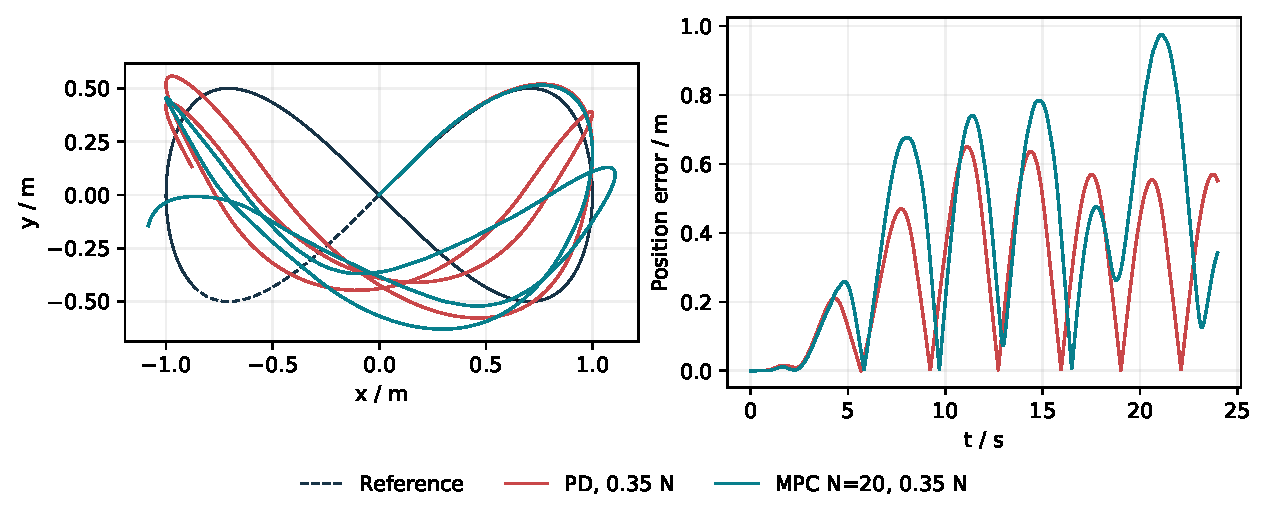
\includegraphics[width=\linewidth]{figures/ch18_mpc.pdf}
\caption{将力限收紧到每轴 0.35 N。两种方法都无法紧贴原参考；MPC 还施加每轴 0.5 m/s 和 2 N/s 约束。
它的失败会切换到制动，因此不能把整条实际输入曲线都称为满足 QP 约束。}
\end{figure}

限力 PD 的 RMS 为 0.3533 m，MPC 为 0.4771 m；MPC 并非所有参数下都更好。
PD 最大速度分量 0.5992 m/s；MPC 约 0.500001 m/s，后者的微小超量在数值容差量级。
MPC 有 21 次 max\_iterations，不能据此断言不可行；制动切换导致实际最大力变化率达 35 N/s。
其最小净空仍有 2.6933 m，但空房间的这次结果不证明任意障碍场景安全。
完整 summary.csv 与 failures.csv 分开记录各次误差、耗时、状态及新的制动力。
